\documentclass[crop,tikz]{standalone}
\usepackage{physics}
\usepackage{amsmath, bm, bbm}
\usetikzlibrary{positioning}
\usetikzlibrary{decorations.pathreplacing,calligraphy}

\usepackage{pgfplots}
\usetikzlibrary{intersections, pgfplots.fillbetween}

\begin{document}
\begin{tikzpicture}[
node/.style={shape=rectangle, rounded corners=.1cm, draw=black, line width=1, fill=black!10},
edge/.style={-latex, thick},
every text node part/.style={align=center}
]

        \node[rotate=90] at (-9, 0) {\Large Test Set};
        \node at (-6, 1.7) {\Large Source\strut};
        \node at (-3, 1.7) {\Large Convergence};
        \node (source) at (-6, 0) {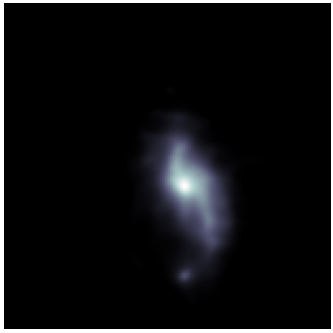
\includegraphics[height=3cm]{source_highlight}};
        \node[color=white] at (-6, 1) {COSMOS};
        \node (kappa) at (-3, 0) {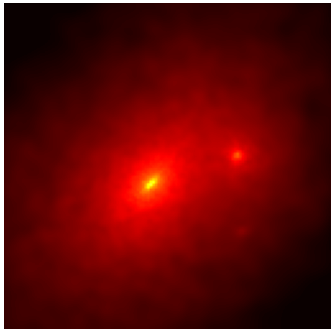
\includegraphics[height=3cm]{kappa_highlight}};
        \node[color=white] at (-3, 1) {Illustris TNG};
        \draw (-7.6, 1.5) .. controls (-7.9, 0.5) and (-7.9, -0.5) .. (-7.6, -1.5);
        \draw (-1.4, 1.5) .. controls (-1.1, 0.5) and (-1.1, -0.5) .. (-1.4, -1.5);
        \node at (-8.2, 0) {\huge $F$};
        \node at (0.75, 0) {\huge $=$};
        \node at (-0.75, 0) {\huge $+$};
        \node at (0, 0) {\huge $\boldsymbol{\eta}$};
        \node at (3, 1.7) {\Large Lensed Image};
        \node (obs) at (3, 0) {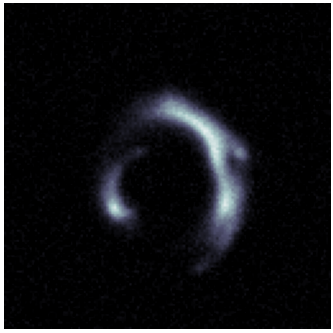
\includegraphics[height=3cm]{observation_highlight}};

        \node[rotate=90] at (-9, -4) {\Large RIM \\ \Large Baseline };
        \node (source_pred) at (-6, -4) {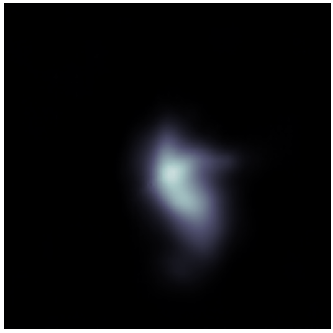
\includegraphics[height=3cm]{source_pred_highlight}};
        \node (kappa_pred) at ( -3, -4) {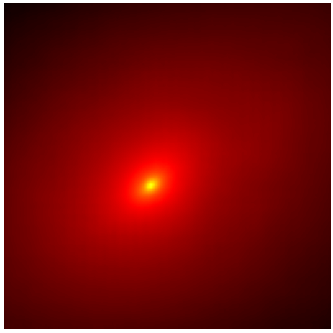
\includegraphics[height=3cm]{kappa_pred_highlight}};
        \node (obs_pred) at (0, -4) {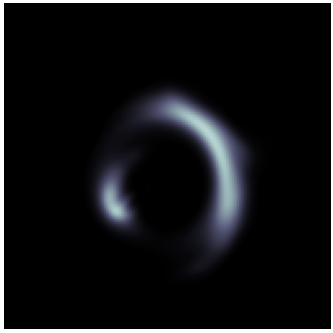
\includegraphics[height=3cm]{observation_pred_highlight}};
        \node (res) at (3, -4) {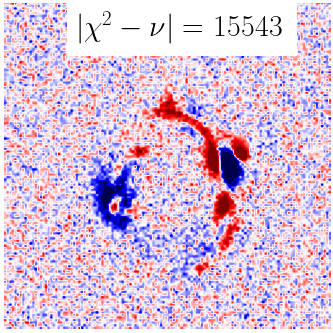
\includegraphics[height=3cm]{residual_highlight}};
        \node at (3, -2.2) {\Large Residuals};

        \node[rotate=90] at (-9, -7) {\Large RIM \\ \Large Fine-Tuned };
        \node (source_pred_reoptim) at (-6, -7) {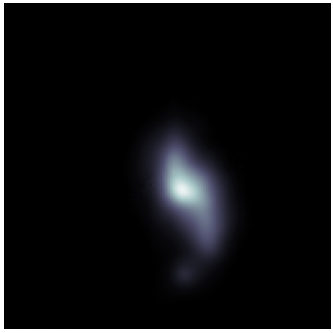
\includegraphics[height=3cm]{source_pred_reoptim_highlight}};
        \node (kappa_pred_reoptim) at (-3, -7) {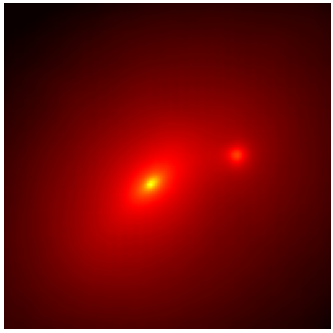
\includegraphics[height=3cm]{kappa_pred_reoptim_highlight}};
        \node (obs_pred_roptim) at (0, -7) {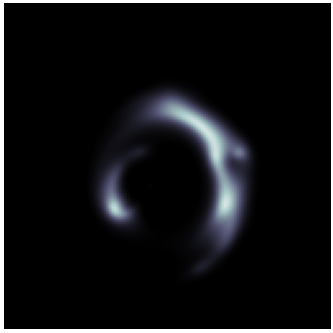
\includegraphics[height=3cm]{observation_pred_reoptim_highlight}};
        \node (res_reoptim) at (3, -7) {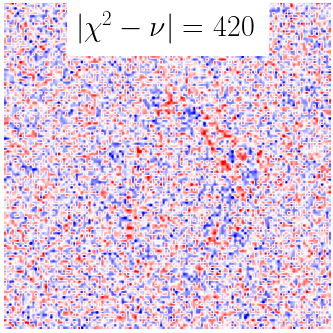
\includegraphics[height=3cm]{residual_reoptim_highlight}};


\end{tikzpicture}
\end{document}
